\chapter{Kriptografske osnove rješenja}
Enkripcija, tj. skriveno pisanje, izvorni je cilj kriptografije\cite{ferguson2011cryptography}, mogućnost tajne komunikacije intrigirala je čovječanstvo tokom poznate historije, te je razvijeno mnoštvo načina da se taj cilj i ostvari, od primitivnih supstitucijskih metoda, pa sve do moderne formalno utemeljene kriptografije\cite{singh2000code}. Kako namjena rješenja u okviru ovog rada diktira, primarni fokus ovog poglavlja biti će međutim stavljen na dodatne mogućnosti moderne kriptografije koje su posebno došle do izražaja razvojem kriptografije javnog ključa i to autentifikaciju entiteta, te utvrđivanje autentičnosti i integriteta poruke, funkcionalnosti poznate i kao digitalni potpis.

\section{Hash funkcije}
Kriptografske hash funkcije igraju ključnu ulogu u savremenoj kriptografiji, njihova osnovna namjena je preslikavanje domena X u uži kodomen Y. Najčešće se koriste u sklopu utvrđivanja integriteta podataka i autentifikacije poruka. Kao ulaz hash funkcije primaju niz bita a kao izlaz vraćaju rezultirajuće preslikavanje koje nazivamo hash-kod, hash-vrijednost ili jednostavno \textbf{hash}\cite{katz1996handbook}, koji je i sam niz bita te se u praksi gotovo uvijek navodi u heksadecimalnom zapisu, npr. \texttt{B0E2B76996D3A488CEFDA9C4B83ECE1E3E49121A}.

\paragraph*{}
Preciznije hash funkcija \textit{h} preslikava niz konačne dužine \textit{n} bita, za domen \textit{D} i kodomen \textit{R} tako da \(h: D \to R\) i \(|D|>|R|\), ovakvo preslikavanje je \textit{many-to-one} i implicira postojanje \textit{kolizija}, tj. različitih parova ulaza sa identičnim izlazom, ovo je nepoželjna ali i neizbježna osobina hash funkcija te se u praktičnim implementacija pokušava minimizirati njen efekat. Osnovna ideja je da hash vrijednost služi kao kraća reprezentativna slika ili digitalni otisak izvornog objekta i koristi se kao da je jedinstveno identifikabilna sa izvornim objektom.

\paragraph*{}
U okviru ovog rada posebno je zanimljiv slučaj korištenja hash funkcija zajedno sa šemama digitalnog potpisivanja u cilju utvrđivanje integriteta podatkovne strukture, gdje se poruka obično prvo hashuje i rezultirajuća hash vrijednost kao reprezent originalne poruke potpisuje korisničkim privatnim ključem. Prema opisanoj definiciji hash funkcija može uzeti mnoštvo oblika, stoga je za bilo kakvu ozbiljniju diskusiju o hash funkcijam potrebno napraviti klasifikaciju njenih različitih oblika koje u zavisnosti od domena primjene uzimaju različite osobine i nameću dodatne zahtjeve i ograničenja, time dajući jasniju sliku o hash funkcijama uopšte. Dvije osnovne osobine svake hash funkcije su:

\begin{itemize}
    \item \textit{kompresija} - funkcija \textit{h} preslikava ulaz \textit{x} proizvoljne konačne dužine \textit{t} niza bita u izlaz \textit{h(x)} fiksne dužine \textit{n} bita
    \item \textit{jednostavnost izračuna} - za datu funkciju \textit{h}, i ulaz \textit{x}, \textit{h(x)} je jednostavna i brza za izračun.
\end{itemize}

\paragraph*{}
Sve hash funkcije zadovoljavaju dvije pobrojane osobine, ali to svojstvo nije dovoljno za njihovu kriptografsku primjenu za koju je neophodno osigurati dodatne garancije, stoga se nameće podjela na nekriptografske i kriptografske hash funkcije, koje dodatno moraju zadovoljiti i najmanje jedan od dva niženavedena uvjeta:

\begin{itemize}
    \item \textit{jednosmjernost} - osigurava da je izračunski teško za datu izlaznu hash vrijednost \textit{y} pronaći izvornu vrijednost parametra \textit{x} hash funkcije \textit{h(x)},
    \item \textit{otpornost na kolizije} - pronalazak dvije iste izlazne hash vrijednosti za dva različita ulazna parametra \textit{x} izračunski je teško i nepraktično, što obično znači da bi za pronalazak kolizije uzevši najbrže trenutno zamislive računare trebalo više vremena nego je proteklo od postanka univerzuma do danas, što se može smatrati razumnom garancijom, koju je kako se je do sada pokazalo praktično teško ispoštovati.
\end{itemize}

\paragraph*{}
Uzevši u obzir sve opisane karakteristike jasno je da broj praktičnih implementacija kriptografskih hash funkcija koje pružaju neophodne garancije relativno mali, no postoje funkcije koje pružaju dovoljno dobre garancije za svakodnevnu praktičnu primjenu, od kojih su najpoznatije SHA, MD i BLAKE familije hash funkcija.

\paragraph*{}
Ilustrativno na slici \ref{fig:hash_dia} dat je prikaz rada SHA-1 hash funkcije za vrijednosti "HAPPYCAT" i "ANGRYCAT", gdje je jednostavno uočljiva različita izlazna hash vrijednost, dodatno navedene vrijednosti bi trebale biti jedinstvene za date ulaze, tj. ne bi smjela postojati neka druga vrijednost osim navedene koja bi dala istu hash vrijednost kao rezultat. SHA-1 funkcija uvijek daje rezultat fiksne dužine 40 bajta. Sa sigurnosnog aspekta relevantno je spomenuti još i to da postoje tabele koje sadrže prethodno izračunate hash vrijednosti za mnoge ulazne parametre i različite funkcije, kao i pretraživače po hash vrijednostima što djelimično narušava garanciju jednosmjernosti, takve tabele nazivaju se \textit{rainbow} tabelama.

\begin{figure}[H]
    \centering
    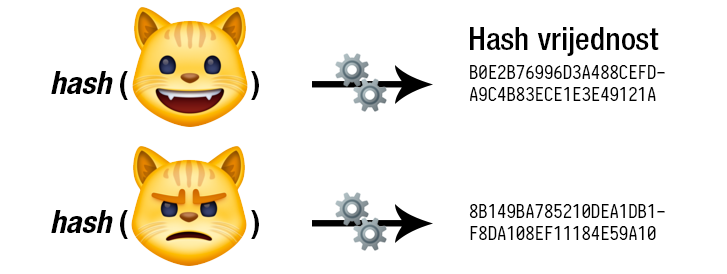
\includegraphics[width=1.0\textwidth]{material/hash_dia}
    \caption{Primjena hash funkcije na dva različita ulazna parametra daje \textbf{različitu i jedinstvenu} izlaznu hash vrijednost za dati ulazni parametar}
    \label{fig:hash_dia}
\end{figure}

\section{Kriptografija javnog ključa}
\textit{Simetrična kriptografija} zahtijeva razmjenu tajnog ključa prije ostvarivanja sigurnog komunikacijskog kanala između dva ili više učesnika, iako vrlo pouzdan metod, često je teško provodiv u praksi, pogotovo u slučajevima ad-hoc i masovne decentralizovane komunikacije nalik internetu, neophodno je da učesnici ili sami izvrše međusobnu razmjenu tajnih ključeva koje će naknadno koristiti ili da jedan autoritativni entitet u kojeg se ima povjerenje to uradi umjesto njih tako što će generisati i distribuirati ključeve svim učesnicima u komunikaciji, očite slabosti ovog modela su da zahtijeva povjerenje i postojanje funkcionalnog sigurnog kanala za razmjenu tajnih ključeva - što često nije slučaj. \textit{Asimetrična kriptografija} ili kriptografija javnog ključa razvijena je sa ciljem prevazilaženja navedenih nedostataka od strane britanske tajne službe GCHQ početkom sedamdesetih godina XX stoljeća, javnosti je naknadno predstavljena kroz radove Merklea\cite{merkle1978secure}, Diffiea i Hellmana\cite{diffie1976new}, a nešto kasnije u obliku danas opštepoznate praktične implementacije RSA kriptosistema Rivesta, Shamira i Adelmana\cite{rivest1978method}, koji dodatno definiše i pojam elektronskog potpisa, kao i njegove komercijalne namjene.

\paragraph*{}
Kriptosistemi javnog ključa uvode ideju dva različita ali povezana ključa, jedan - javni samo za enkripciju i jedan - privatni samo za dekripciju, a kako nije moguće saznati jedan ključ iz drugog korisnik je slobodan javno objaviti svoj ključ za enkripciju, tako da ukoliko npr. Alisa želi poslati tajnu poruku Bobu, dovoljno je da posjeduje Bobov sada \textit{javni enkripcijski ključ} i da ga iskoristi da njime šifruje poruku. Kada Bob primi takvu poruku iskoristiti će svoj \textit{tajni privatni ključ} i dešifrovati Alisinu poruku, kompletna interakcija i sastavni elementi prikazani su na slici \ref{fig:alice_bob_enc}.

\begin{figure}[H]
    \centering
    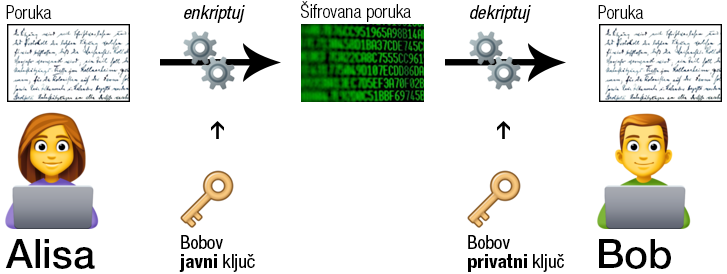
\includegraphics[width=1.0\textwidth]{material/bob_alice_enc}
    \caption{Tajna komunikacija unutar javnog kriptosistema}
    \label{fig:alice_bob_enc}
\end{figure}

\paragraph*{}
Kriptografija javnog ključa ne osigurava samo tajnost komunikacije kao u opisanom slučaju, nego se može koristiti i za potvrdu autentičnosti. Za takav scenario dovoljno je da Bob svojim privatnim ključem \textit{potpiše} željenu poruku ili datotetu i Alisa će biti u mogućnosti da provjeri da je ta poruka autentično kreirana od strane Boba, za tu namjenu potrebno je da Alisa posjeduje Bobov javni ključ od ranije ili da ga dobavi iz nekog povjerljivog izvora jer mora biti sigurna da neko lažno ne podmetne svoj ključ kao Bobov, više o ovoj namjeni asimetričnih kriptosistema biti će dato u zasebnom poglavlju u nastavku, no za sada je bitno imati je na umu. Spomenuti proces potpisivanja sastoji se od par kriptografskih operacija, vrlo sličnih kriptovanju poruke, no kako u ovom slučaju nije potrebno prenijeti kompletan sadržaj nego samo omogućiti verifikaciju, proces je moguće učiniti efikasnijim tako što će se poruka prije obrade privatnim ključem prethodno provući kroz neku od hash funkcija, koja će poruku znatno smanjiti i ubrzati sam proces, detaljan prikaz dat je u poglavlju \ref{subs:dsig}.

\subsection{Sigurnosni ciljevi}
Sigurnosni ciljevi kriptografije javnog ključa pored povjerljivosti, kao primarne funkcije, kako je već i pomenuto, uključuju i mogućnosti za provjeru integriteta i autentičnosti poruke, autentifikacija entiteta, te osiguravanje neporecivosti izvršene akcije\cite{buchmann2013introduction}, ovakav jedinstven i širok skup funkcionalnosti kriptografiji javnog ključa daje fundamentalni značaj u modernim digitalnim komunikacijama i internet poslovanju, stoga su osnovne karakteristike svakog od navedenih ciljeva ukratko opisane u nastavku.

\subsubsection*{Povjerljivost i privatnost}
Povjerljivost je osnovni sigurnosni cilj kriptografije i odnosi se na osobinu da tajni podaci neće biti dostupni neautorizovanim osobama. Povjerljivost omogućava privatnost i međusobno su usko povezane. Privatnost označava sposobnost očuvanja vlastitih podataka tajnim za sve one koji nisu eksplicitno autorizovani za njihov pregled i predstavlja osnovno ljudsko pravo garantovano članom 12 Univerzalne deklaracije o ljudskim pravima\cite{assembly1948universal}:

\begin{quote}
\textit{"Niko ne smije biti podvrgnut samovoljnom miješanju u njegovu privatnost, obitelj, dom ili dopisivanje, niti napadima na njegovu čast i ugled. Svako ima pravo na zakonsku zaštitu protiv takvog miješanja ili napada."}
\end{quote}

\paragraph*{}
Mnoštvo je primjera važnosti povjerljivosti i privatnosti u savremenoj eri opšteprisutne digitalizacije i internet poslovanja, nažalost narušavanje ovih temeljnih vrijednosti postalo je gotovo normalna i svakodnevna pojava bilo da se radi o krađi osjetljivih podataka i digitalnih dobara od strane malicioznih agenata ili prisluškivanju od strane korporativnih i vladinih agencija koje vrše masovno špijuniranje na globalnom nivou prikupljanjem privatnih podataka putem raznovrsnih skrivenih programa nadzora i praćenja\cite{wleaks}.

\subsubsection*{Autentifikacija entiteta}
Autentifikacija se odnosi na proces utvrđivanja stvarnog identiteta, navedeni identitet može se odnositi na osobu, kompaniju ili bilo koji drugi koncept koji se od drugog razlikuje po sebi svojstvenim osobinama. Za isti proces može se približno precizno koristiti i termin identifikacija. Poznavanje identiteta u okviru digitalnog okruženja često je neophodno za ispravno funkcionisanje programskog rješenja i pravilnu raspodjelu autorizacija, kao i za relacije povjerenja između različitih kategorija korisnika. Često se za ovu namjenu koriste korisnička imena i lozinke kao najprostiji vid implementacije, no mnogo su pouzdaniji namjenski izrađeni repozitoriji identiteta ili infrastrukture javnih ključeva (\textit{PKI - public key infrastructure}), koji omogućavaju mnogo sigurniju autentifikaciju, bolje provođenje dobrih sigurnosnih praksi, širi spektar primjene i bolju integraciju. Aplikacija izrađena u okviru ovog rada sadrži namjenski izrađen pokazni repozitorij identiteta i javnih ključeva u vidu Logit API implementacije.

\subsubsection*{Integritet i autentičnost poruke}
Integritet se odnosi na garanciju da podaci nisu mijenjani nakon što ih je izvorni autor sačinio, mnoštvo je bitnih aktivnosti gdje je upravo ovakva garancija od iznimne važnosti. Koncept integriteta dodatno se proširuje kroz pojam autentičnosti poruke, gdje se zahtijeva i mogućnost utvrđivanja njenog izvorišta, te njegova autentifikacija. Ove aktivnosti izvode se putem digitalnog potpisivanja i vjerodostojnih repozitorija koji sadrže provjerene identitete entiteta.

\paragraph*{}
Kao primjer možemo uzeti svakodnevno poznate korisničke scenarije, svaki računarski program ili nadogradnja kada se distribuira krajnjim korisnicima može biti naknadno izmijenjen u cilju izvršavanja određenih zlonamjernih aktivnosti koje mogu naštetiti korisniku, da bi se ovo izbjeglo većina savremenih operativnih sistema podržava određeni način provjere integriteta softvera prilikom instalacije na korisničkom računaru i autentičnost identiteta njenog izvorišta, ovakve provjere posebno su bitne u sigurnosno osjetljivim okruženjima i djalatnostima gdje bi pokretanje zlonamjernog koda moglo ugroziti živote ili uzrokovati veliku materijalnu štetu, primjeri takvih sistema su računari u zdravstvu i kontrolni sistemi javnih infrastruktura, poput aerodroma, električne ili vodovodne mreže, no nikako ne treba zanemariti i kućne korisnike koji su itekako izloženi raznim vrstama sigurnosnih prijetnji. Za namjene utvrđivanja integriteta i autentifikacije izvorišta programskih rješenja održavaju se repozitoriji sa identitetima softverskih razvojnih kuća i njihovim ključevima.

\paragraph*{}
Utvrđivanje integriteta poruke i autentifikacija učesnika se koristi u okviru aplikacije za bilježenje prisustva studenata predložene u okviru ovog rada na način da se potpisano vrijeme i lokacija svih studentskih uređaja dodatno potpisuje predavačkim ključevima unutar jedinstvene sesije (npr. nastavnog časa) koju po zaključenju nije moguće naknadno mijenjati bez narušavanja integriteta navedene sesije. Identitet svih učesnika i autentičnost njihovih potpisa provjerava se korištenjem namjenskog repozitorija na Logit API.

\subsubsection*{Neporecivost}
Neporecivost je osobina podataka koja sprječava poduzimača određene aktivnosti da istu porekne nakon njenog okončanja, npr. slanje poruke, novčana transakcija ili prisustvo predavanju. Kod primjera prisustva, radi se o nemogućnosti studenta da nakon što digitalno prijavi svoje prisustvo na predavanju unutar predložene Logit NFC aplikacije naknadno to prisustvo porekne jer postoji jedinstveni digitalno potpisan trag koji to dokazuje, za čvrst dokaz neophodno je osigurati i jaku povezanost korisnika i nosioca identiteta - u ovom slučaju mobilnog uređaja, za ovakve namjene posebno su pogodne višefaktore metode identifikacije koje uključuju i biometrijske osobine.

\section{RSA kriptosistem}
Rivest, Shamir i Adelman\cite{rivest1978method} predložili su kriptosistem koji može osigurati osobine privatnosti i potpisivanja poruka ekvivalentne ili bolje od onih kakve posjeduje papirna pošta. Njihov sistem baziran je na konceptu sistema javnog ključa kakav su ranije opisali Diffie i Hellman\cite{diffie1976new}. Sveukupna procedura sastoji se od procesa enkripcije \textit{E}, procesa dekripcije \textit{D} i izvorne nešifrovane poruke \textit{M}, te za takav sistem mora da vrijedi:

\begin{enumerate}
  \item dešifrovanje kriptovane forme poruke \textit{M} daje \textit{M}, \[D(E(M)) = M\]
  \item i \textit{E} i \textit{D} su jednostavne za izračun,
  \item javno obznanjujući \textit{E} korisnik ne otkriva jednostavan način za izračun \textit{D}. Praktično ovo znači da samo on može dekriptovati poruke kriptovane pomoću \textit{E}
  \item ukoliko je poruka \textit{M} prvo dešifrovana a onda šifrovana, rezultat je \textit{M}, \[E(D(M)) = M\]
\end{enumerate}

\paragraph*{}
Enkripcijska procedura se sastoji od \textit{opšte metode} i \textit{enkripcijskog ključa}. Opšta metoda, pod kontrolom ključa, šifruje poruku \textit{M} i rezultira šifrovanom porukom \textit{C (en. ciphertext)}. Svako može koristiti istu opštu metodu (algoritam), jer sigurnost procedure u potpunosti počiva na sigurnosti seta ključeva. Stoga otkrivanje enkripcijske procedure tada znači i objavu \textit{javnog} ključa.

\paragraph*{}
Efektivno kada korisnik otkrije \textit{E}, on otkriva vrlo neefikasan način izračuna \textit{D(C)} testiranjem svih mogućih poruka \textit{M} sve dok se ne nađe ona koja zadovoljava \(E(M) = C\). Ukoliko je osobina (3) zadovoljena broj takvih poruka nije praktičan za izračun.

\paragraph*{}
Funkcija \textit{E} ukoliko zadovoljava osobine (1)-(3) predstavlja tzv. \textit{"jednosmjernu funkciju sa stupicom"}, a ukoliko zadovoljava i (4) onda je \textit{"jednosmjerna permutacija sa stupicom"}. Diffie i Hellman\cite{diffie1976new} uveli su koncepte jednosmjernih funkcija sa stupicom ali nisu dali implementaciju. Ove funkcije nazivaju se jednosmjernim jer ih je jednostavno izračunati u jednom smijeru ali bi trebalo biti vrlo teško u suprotnom, dok su "sa stupicom" jer su njihovi inverzi jednostavni za izračun ukoliko je poznata određena informacija, u slučaju šifrovanja je to privatni ključ. Ovakva funkcija koja također zadovoljava i (4) mora biti permutacija: svaka poruka je ciphertekst neke druge poruke i svaki ciphertekst je dozvoljena poruka. Zadovoljenje osobine (4) neophodno je za implementaciju potpisivanja.

\subsection{Ključevi i komunikacija} \label{subs:keygen}
Da bi kreirali vlastite privatne i javne ključeve učesnici moraju svaki za sebe i nasumično odabrati dva velika prosta broja \textit{p} i \textit{q} takva da nije vjerovatno da računar može izvršiti cjelobrojnu faktorizaciju \(n = p * q\), danas se minimalno preporučuju brojevi sličnog reda veličine koji daju proizvod dužine 2048 bita kao sigurni do 2030. godine\cite{kaliski2003twirl}. Proizvod \textit{n} postaje dijelom javnog ključa, dok se pojedinačni faktori moraju čuvati u tajnosti zbog njihovog korištenja u derivaciji privatnog ključa.

\paragraph*{}
Korisnici također moraju izabrati i cjelobrojnu vrijednost \textit{e} takvu da, \[1 < e < \phi(n) = (p - 1)(q - 1) \wedge \gcd(e, (p - 1)(q - 1)) = 1.\] Obratite pažnju da je \textit{e} uvijek neparno jer je \((p - 1)(q - 1)\) parno. Dalje korisnik računa cjelobrojnu vrijednost \textit{d}, \[1 < d < (p - 1)(q - 1) \wedge de \equiv 1\bmod(p - 1)(q - 1).\] Korisnikov javni ključ sada je par \textit{(n, e)}, dok je njegov privatni ključ \textit{d}. Broj \textit{n} naziva se \textit{RSA modulus}, \textit{e} je \textit{enkripcijski eksponent}, a \textit{d - dekripcijski eksponent}\cite{buchmann2013introduction}.

\paragraph*{}
Ponovno se može poslužiti primjerom Boba i Alise opisanim ranije, sada se može reći da kada je Bob korištenjem opisane procedure generisao neophodne vrijednosti ključeva i poslao Alisi svoj javni ključ, tj. vrijednosti \textit{(n, e)}, koje će ona iskoristiti za šifrovanje proizvoljne poruke \textit{m}, što sada možemo izraziti kao \[c = m^e\bmod n.\] Kada Bob primi Alisinu šifrovanu poruku \textit{c} iskoristiti će tajnu vrijednost \textit{d} i dešifrovati poruku \[m = c^d\bmod n.\]

\subsection{Digitalni potpis} \label{subs:dsig}
Digitalni potpis osigurava mehanizam provjere integriteta i u kombinaciji sa adekvantnom infrastrukturom - autentičnost izvorišta poruke. Ukoliko Bob želi potpisati određeni dokument, on korištenjem svog privatnog ključa izračunava jedinstveni niz bita, koji Alisi garantuje da će korištenjem Bobovog prethodno dobavljenog javnog ključa moći verifikovati da navedeni dokument nije izmijenjen u putu do nje, kao i da je Bob originalni potpisnik dokumenta, navedena interakcija prikazana je na slici \ref{fig:alice_bob_sig}, dodatno Bob u budućnosti ne može poreći da je potpisao navedeni dokument, što osigurava još jednu vrlo bitnu funkcionalnost cjelokupnog sigurnosnog sistema. Ovakav sistem predstavlja temelj na kojem je izgrađen siguran internet i digitalna ekonomija te je duboko utkan u osnovne protokole poput TLS, SSH, PGP etc.\cite{dierks2008transport}

\begin{figure}[H]
    \centering
    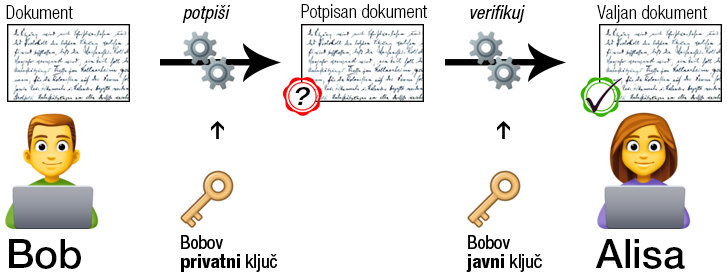
\includegraphics[width=1.0\textwidth]{material/bob_alice_sig}
    \caption{Verifikacija integriteta i autentičnosti uz garancija neporecivosti u okviru javnog kriptosistema}
    \label{fig:alice_bob_sig}
\end{figure}

\paragraph*{}
RSA šema najčešće je korišten algoritam digitalnog potpisivanja. Generisanje ključeva funkcionira na istom principu kao i u primjeru šifrovanja poruke opisanom u poglavlj \ref{subs:keygen}. Svaki digitalni potpis zavisan je od sadržaja poruke i potpisnika, u protivnom bilo bi moguće da isti potpisnik koristi jedan potpis za više dokumenata, što ovdje nije slučaj. Da bi se uspješno implementiralo digitalno potpisivanje, kriptosistem mora zadovoljavati osobine spomenute jednosmjerne permutacije sa stupicom, budući da će dekripcijski algoritam biti primjenjivan na izvorni - nešifrovan dokument.

\paragraph*{}
Opisani primjer razmjene potpisanog dokumenta ili poruke \textit{M} između Alise i Boba može se unutar RSA kriptosistema preciznije prikazati kao: \[S = D_{B}(M),\] gdje je \textit{S} digitalno potpisana poruka a \(D_{B}\) Bobova funkcija za dešifrovanje korištenjem privatnog ključa. Kako je već napomenuto primjena funkcije za dešifrovanje na nešifrovanu poruku ima smisla u slučaju da kriptosistem zadovoljava potrebne uvjete. Ukoliko je dodatno potrebno osigurati i tajnost potpisane poruke Bob je može naknadno šifrovati Alisinim javnim ključem, u tom slučaju Alisa po prijemu prvo vrši dešifrovanje svojim privatnim ključem da bi dobila Bobovu izvornu potpisanu poruku \textit{S}, korištenjem Bobovog javnog ključa Alisa sada "šifruje" potpisanu poruku \[M = E_{B}(S)\] time dolazeći u posjed uređenog para \textit{(M, S)} sa osobinama sličnim onima koje ima originalni fizički potpisan dokument.

\paragraph*{}
Sama praktična implementacija potpisivanja razlikuje se međutim od opisane procedure u tome da se u praksi ne vrši potpisivanje cjelokupne izvorne poruke, nego se nad njom prvobitno korištenjem kriptografske hash funkcije izračunava jedinstvena hash vrijednost, pa Bob tako umjesto poruke potpisuje dobijenu hash vrijednost svojim privatnim ključem, dok na drugom kraju Alisa ponavlja proces izračunavanja hash vrijednosti koristeći Bobovu izvornu poruku, njegov javni ključ i istu hash funkciju, te dobijeni hash poredi sa Bobovim hashom, u slučaju poklapanja hash vrijednosti Alisa može biti sigurna u valjanost digitalnog potpisa. Jedina funkcionalna razlika ovakvog pristupa je da se koncept poruke ili dokumenta, odvaja od samog digitalnog potpisa, što olakšava rad i osigurava dodatne sigurnosne i upotrebne prednosti.

\paragraph*{}
Praktična implementacija može se formalno opisati kao primjena hash funkcije \textit{h} tako da potpis \textit{s} niza karaktera poruke \(m \in \lbrace 0,1\rbrace ^n\) glasi \[s = h(m)^d\bmod n.\] \textit{d} je u prikazanom slučaju Bobov \textit{dekripcijski eksponent}. Da bi Alisa verifikovala zaprimljeni potpis \textit{s} koristi Bobov javni ključ \textit{(n, e)} i izračunavanjem hash vrijednost \textit{h(m)} poruke \textit{m} i vrši provjeru \[h(m) = s^e\bmod n.\] Potpis je valjan ako i samo ako važi data jednakost. Za potrebe Logit sistema korištena je SHA-256 hash funkcija u kombinaciji sa RSA potpisom.

\pagebreak[4]

\section{PKI - infrastruktura javnog ključa}
Iako kriptografija javnog ključa ne zahtijeva razmjenu tajnih ključeva da bi se ostvarila povjerljiva komunikacija, vrlo je bitan aspekt upravljanja ključevima, kako javnim tako i privatnim. Namjena infrastrukture javnog ključa \textit{en. PKI - public key infrastructure} je efikasno i sigurno upravljanje ključevima tokom njihovog životnog ciklusa.

\subsection{Životni ciklus ključeva}
Životni ciklus ključeva počinje od samog generisanja, kako je opisano u poglavlju \ref{subs:keygen}, nakon čega slijedi upotrebni vijek tokom kojeg se privatni ključevi koriste za potpisivanje ili dešifrovanje primljenih poruka. Korisnici također imaju pristup javnim ključevima drugih korisnika, te ključeve koriste za šifrovanje ili verifikaciju potpisanih dokumenata. U završnoj fazi ključevi izlaze iz upotrebe bilo putem zastarijevanja ili kroz neki drugi događaj. Svaka od pomenutih faza u životnom ciklusu para ključeva mora imati određene procedure koje osiguravaju provođenje dobrih praksi u upravljanju ključevima.

\subsubsection{Generisanje i pohrana}
Osnovni preduvjet za generisanje sigurnog para ključeva je osiguravanje pouzdanog okruženja, najbolje je da tu aktivnost izvode sami korisnici, jer u tom slučaju privatni ključ ne bi trebao biti dostupan nijednoj trećoj strani, što u praksi često nije slučaj, budući da korisničko okruženje može biti kompromitovano ili na neki drugi način neadekvatno za tu namjenu, stoga se često mora pribjeći generisanju ključeva u okruženju neke povjerljive treće strane za koju se može biti sigurno da ključeve neće zloupotrijebiti. Pored navedenog i samo skladištenje ključeva, posebno privatnih, pruža mnoge sigurnosne izazove. Uzimajući u obzir nabrojano jasno je da navedenim problemima treba pristupiti planski i krajnje ozbiljno jer u protivnom sigurnost kompletnog sistema može biti kompromitovana od samog početka. Logit aplikacija privatne ključeve generiše i pohranjuje isključivo unutar Android repozitorija ključeva na korisničkom uređaju, za koji postoje garancije nemogućnosti ostvarenja pristupa korištenjem bilo koje druge aplikacije.

\subsubsection{Upotrebni vijek}
Tokom upotrebne faze životnog vijeka ključeva osnovna funkcionalnost je obezbijediti siguran pristup korisničkim javnim ključevima. Pored toga, u cilju pružanja adekvatnih garancija identiteta i potvrde autentičnosti neophodno je utvrditi i provesti jasne procedure koje će osigurati neupitnu povezanost entiteta/osoba sa ključevima, u protivnom može doći do krađe identiteta i lažnog predstavljanja. Logit API vrši funkciju repozitorija javnih ključeva za korisnike sistema i povezuje korisnike sa njihovim ključevima, osigurana je osnovna provjera identiteta putem korisničke prijave na fakultetski ZAMGER sistem.

\subsubsection{Kraj životnog ciklusa}
Dodatno je potrebno utvrditi procedure za kraj životnog vijeka i pohranu starih ključeva. Kod Logit API repozitorija ne postoji vremenski ograničen vijek trajanja para ključeva, no pri svakoj novoj instalaciji aplikacije ili zamjeni uređaja, stari par ključeva se arhivira a novogenerisani ključevi se koriste kao sigurnosno relevantni. Pored navedenih funkcionalnosti Logit API se koristi i kao repozitorij potpisanih dokumenata, u ovom slučaju, prisustava predavanjima, no to izlazi iz okvira PKI i može se smatrati dodatnom funkcionalnošću.

\subsection{Hijerarhija povjerenja}
Za praktičnu upotrebu kriptografije javnog ključa neophodno je da korisnici vjeruju u autentičnost dostupnih javnih ključeva. Stoga su pored prostog direktnog modela povjerenja sa dva učesnika koji razmjenjuju sopstvene javne ključeve uspostavljene raznovrsne hijerarhije povjerljivih učesnika koje omogućavaju formiranje složene mreže koja i sama kao svoju osnovu koristi digitalni potpis i dostupne kriptografske metode.

\paragraph*{}
Primjer jedne složene hijerarhije povjerenja prikazan je na slici \ref{fig:pki}, u ovakvom modelu javne ključeve svih nižih učesnika potvrđuje CA \textit{(en. certification authority)}, koji ujedno na adekvatan način vrši i verifikaciju autentičnosti. Većina ovakvih hijerarhijskih PKI arhitektura uređena je u skladu sa standardom X.509. U ovakvom okruženju može da učestvuje više nivoa posrednih CA \textit{(en. intermediate CA)} i obično je uređeno u strukturu drveta sa listovima, gdje se u korijenu nalazi CA \textit{(en. root CA)} kojeg svi posredni CA uzimaju kao pouzdanog i koji sam potpisuje svoj certifikat. Na dnu strukture drveta nalaze se krajnji korisnici kriptosistema. Da bi se ostvarila relacija povjerenja između dva korisnika, nije neophodno da oni dijele isti posredni CA, dovoljan uslov je da se može napraviti veza prema jednom CA u kojeg oba korisnika imaju povjerenje da bi pomenuta relacija bila zadovoljena.

\begin{figure}[H]
    \centering
    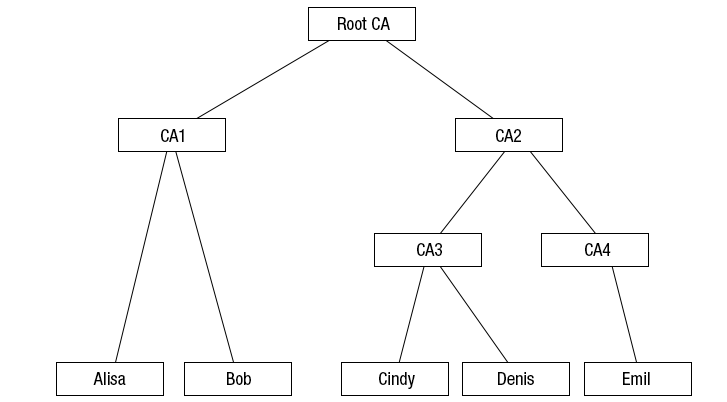
\includegraphics[width=1.0\textwidth]{material/pki}
    \caption{Primjer hijerarhijske infrastrukture javnog ključa}
    \label{fig:pki}
\end{figure}

\paragraph*{}
Primjer jedne relacije povjerenja iz priložene hijerarhije može se formirati između korisnika Alisa i Emil, gdje se može jasno utvrditi \textit{certifikacijska putanja} koja za oba korisnika seže do korijenskog Root CA, ilustrativno za Alisu i Emila važi: \[Alisa \to CA1 \to Root CA\] \[Emil \to CA4 \to CA2 \to Root CA\] Dubina certifikacijske putanje također može da igra ulogu u zavisnosti od različitih zahtjeva, u nekim slučajevima, duže putanje, poput Emilove - se mogu smatrati nepouzdanim za određene namjene, u svakom slučaju poželjno je korištenje što bližih međusobnih putanja.

\paragraph*{}
Logit API posjeduje svoj set ključeva kojim potpisuje sve zaprimljene korisničke sesije prisustva. Da bi se upotpunio model povjerenja neophodno je da se LAPI certifikat potvrdi od strane institucije koja implementira navedeni sistem, u ovom slučaju Elektrotehničkog fakulteta, koja je dalja poveznica na vanjski korijenski CA i omogućava izgradnju šireg sistema povjerenja gdje više institucija koje koriste isti sistem može ostvariti posredne relacije povjerenja. Važno je istaknuti također da korisnici registracijom bivaju uključeni u LAPI repozitorij, što se može smatrati ekvivalentom certifikata, dodatno korisnici (student, nastavnik) obostrano potvrđuju prisustvo a samim tim ostvaruju i direktnu vezu povjerenja, jer aktivnost prikupljanja potpisa podrazumijeva međusobnu identifikaciju korisnika. Prikaz takvog modela dat je na slici \ref{fig:logit_pki}.

\begin{figure}[H]
    \centering
    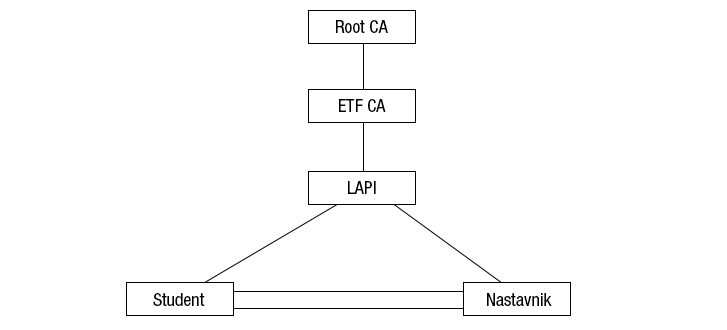
\includegraphics[width=1.0\textwidth]{material/logit_pki}
    \caption{Prikaz Logit PKI hijerarhije}
    \label{fig:logit_pki}
\end{figure}

\subsection{Certifikati}
Bitan aspekt PKI je garancija autentičnosti javnih ključeva, jedan od načina ostvarenja takve garancije su svakako certifikati, tj. strukture koje povezuju javne ključeve sa entitetima ili osobama, najčešće su pohranjeni na PKI koji se brinu da uz pomoć identifikacijskih procedura osiguraju što jaču relaciju između samog entiteta i javnog ključa. U cilju iskoristivosti neophodno je da certifikati obezbijede određeni nivo tehničkih i domenski relevantnih podataka, u većini slučajeva to su:

\begin{itemize}
    \item ime ili naziv entiteta za čiji javni ključ je vezan
    \item javni ključ entiteta
    \item korišteni kriptografski algoritam
    \item serijski broj
    \item period važenja
    \item naziv izdavača certifikata, koji je ujedno i potpisnik
    \item namjena i ograničenja korištenja javnog ključa
\end{itemize}

\paragraph*{}
Sam sadržaj certifikata u većini slučajeva je standardizovan, danas najčešće standardom X.509, gdje i izdati certifikati u skladu sa standardom nose naziv X.509 certifikati, primjer jednog takvog certifikata dat je na slici \ref{img:etf_cert_gen}, navedene su osnovne informacije o certifikatu i opšte informacije pobrojane iznad, dodatno na slici \ref{img:etf_cert_tree} prikazana je certifikacijska putanja datog certifikata. Pored navedenih informacija certifikat obično sadrži i mnoštvo drugih informacija, budući da standard dopušta proširivanje da bi obuhvatio širok domen primjene. Bitno je još napomenuti da zbog vrlo široke primjene u različitim programskim rješenjima postoji mnoštvo različitih formata zapisivanja i razmjene samih certifikata, te je često neophodno konvertovati certifikate u jedan od odgovarajućih formata.

\paragraph*{}
X.509 certifikati koriste ASN.1 \textit{(en. abstract syntax notation version 1)} kao jezik za izvornu specifikaciju osobina certifikata, pomoću navedenog jezika moguće je izraziti mnoštvo kompleksnih struktura za opis osobina certifikata, jedan od mnoštva načina da se navedena specifikacija zapiše je DER \textit{(en. distinguished encoding rules)}, koja je dalje bazirana na BER pravilima za zapisivanje \textit{(en. basic encoding rules)}, navedene strukture predstavljaju svojevrsnu hijerarhiju deskriptivnih jezika i meta-jezika.

\begin{figure}[H]
    \centering
    \begin{subfigure}{.5\textwidth}
        \centering
        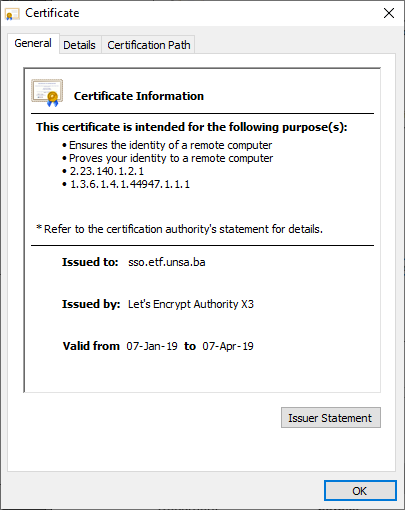
\includegraphics[width=1\textwidth]{material/etf_cert_gen}
        \caption{opšte karakteristike}
        \label{img:etf_cert_gen}
    \end{subfigure}%
    \begin{subfigure}{.5\textwidth}
        \centering
        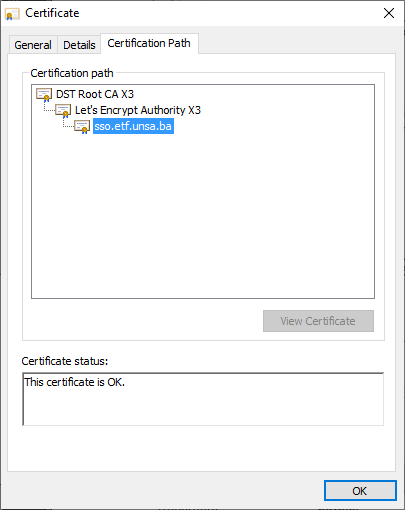
\includegraphics[width=1\textwidth]{material/etf_cert_tree}
        \caption{lanac povjerenja}
        \label{img:etf_cert_tree}
    \end{subfigure}
    \caption{Osobine certifikata}%
    \label{img:etf_cert}
\end{figure}

\paragraph*{}
Logit aplikacija interno koristi namjenski i nestandardni format certifikata, no sve LAPI i korisničke certifikate moguće je pretvoriti u bilo koji od standardnih formata i tako ostvariti interakciju sa ostalim sistemima ukoliko se za to ukaže potreba. Dovoljno je na Logit API strani implementirati novu URI lokaciju koja bi vraćala certifikate u standardizovanom formatu.